%
% teil1.tex -- Beispiel-File für das Paper
%
% (c) 2020 Prof Dr Andreas Müller, Hochschule Rapperswil
%
% !TEX root = ../../buch.tex
% !TEX encoding = UTF-8
%
\section{Musterbildung in Reaktionsdiffusionssystemen
\label{reaktdiff:section:teil1}}

In diesem Abschnitt wird die Reaktionsdiffusionsgleichung mit zwei Komponenten untersucht.
Als Beispiel wurde sich hier für die Turing-Muster entschieden.
Turing-Muster findet man häufig in der Natur zum Beispiel als Fellmuster bei Tieren oder  das Muster unserer Fingerabdrücke.
Sie sind nach dem Mathematiker Alan Turing benannt, der sie 1952 in seinem Artikel \textit{The Chemical Basis of Morphogenesis} \cite{turing1952chemical} beschrieb.
Er untersuchte Systeme, die aus zwei Komponenten bestehen, einem Inhibitor und einem Aktivator.
Turing entdeckte für die Entstehung der Turing-Muster eine Bedingung, die sogenannte Turing Bedingung.
Sie besagt, dass ein System, in welchem Turing-Muster entstehen können, in Abwesenheit von Diffusion stabil sein muss und mit Diffusion instabil wird.
Diese Kapitel basiert auf \cite{reaktdiff:turing_patterns_2019} und \cite{reaktdiff:hoyle2006pattern}.

\subsection{Lineare Stabilitätsanalyse ohne Diffusion
\label{reaktdiff:subsection:mathe}}
Als Basis haben wir zwei Komponenten \(u\) und \(v\).
Die Reaktionsdiffusionsgleichungen für \(u\) und \(v\) lauten
\begin{align*}
    %\label{reaktdiff:equation:reaktdiff1}
    \frac{\partial u}{\partial t} &= D_u \Delta u + f(u,v)\\
    \label{reaktdiff:equation:reaktdiff2}
    \frac{\partial v}{\partial t} &= D_v \Delta v + g(u,v),
\end{align*}
wobei \(D_u, D_v > 0\) die Diffusionskoeffizienten der Komponenten \(u\) und \(v\) sind.

\subsubsection{Statische Lösung}
Als erstes wird der erste Teil der Turing-Bedingung untersucht welcher besagt, dass ein System ohne Diffusion stabil sein muss.
Hierfür wird eine lineare Stabilitätsanalyse ohne Diffusion durchgeführt.
Man betrachte die Gleichungen
\begin{equation}
    \label{reaktdiff:equation:reaktdiff2ohneDiff}
    \frac{\partial u}{\partial t} = f(u_0,v_0),\,
    \frac{\partial v}{\partial t} = g(u_0,v_0).
\end{equation}

\subsubsection{Linearisierung}
Im Fokus liegt die stationäre Lösung \(u_0, v_0\) der Gleichungen \eqref{reaktdiff:equation:reaktdiff2ohneDiff}, das heisst dass \(f(u_0,v_0) = g(u_0,v_0) = 0\).
Nun wird eine kleine Störung $\delta$ zu $u_0$ und $v_0$ hinzugefügt, sodass gilt
\begin{align*}
    u &= u_0 + \delta u\\
    v &= v_0 + \delta v,
\end{align*}
wobei $\delta$ klein ist, das heißt $\delta \ll 1$.
Jetzt kann man die Reaktionsterme linearisiern.
Hierfür nutzt man die Taylor-Entwicklungen bis zum linearen Term.
Sie werden zu
\begin{align*}
    f(u,v) &\approx f(u_0,v_0) + f_u  u + f_v v\\
    g(u,v) &\approx g(u_0,v_0) + g_u  u + g_v v.
\end{align*}
Hierbei sind \(f_u, f_v, g_u, g_v\) die partiellen Ableitungen von \(f\) und \(g\) nach \(u\) und \(v\).
Die Terme \(f(u_0,v_0)\) und \(g(u_0,v_0)\) sind Null, da \(u_0\) und \(v_0\) stationäre Lösungen sind.
Nun können die Gleichungen \eqref{reaktdiff:equation:reaktdiff2ohneDiff} umgeschrieben werden zu
\begin{align}
    \label{reaktdiff:equation:reaktdiff2ohneDifflinearisiert1}
    \frac{\partial u}{\partial t} &= f_u u + f_v v\\
    \label{reaktdiff:equation:reaktdiff2ohneDifflinearisiert2}
    \frac{\partial v}{\partial t} &= g_u u + g_v  v.
\end{align}
Diese Gleichungen sind lineare partielle Differentialgleichungen.
Die Frage ist nun, wie sich die Störungen \(u\) und \(v\) mit der Zeit entwickeln, werden sie grösser oder kleiner.
Wenn man sie in Matrixform schreibt, erhält man
\begin{equation*}
    \label{reaktdiff:equation:reaktdiff2ohneDiffmatrix}
    \frac{\partial}{\partial t} \begin{pmatrix}
        \delta u\\
        \delta v
    \end{pmatrix} = 
    J 
    \begin{pmatrix}
        \delta u\\
        \delta v
    \end{pmatrix}
    , \quad
    J =
    \begin{pmatrix}
        f_u & f_v\\
        g_u & g_v
    \end{pmatrix}.
\end{equation*}
Die Matrix \(J\) ist die Jacobi-Matrix der Reaktionsgleichungen.

\subsubsection{Stabilität}
Damit die Gleichung stabil ist, müssen die Eigenwerte der Matrix \(J\), negative Realteile haben.
Hierbei ist es ausreichend dass die Spur \(\text{Tr}(J) < 0\) und die Determinante \(\det(J) > 0\) sind.
Das kann man zeigen, indem
\begin{equation*}
    \det(A - \lambda I) = 0
\end{equation*}
gelöst wird, wobei \(I\) die Einheitsmatrix ist.
Die Eigenwerte der Matrix \(J\) sind die Lösungen der Gleichung
\begin{equation*}
    \lambda^2 - \text{Tr}(J) \lambda + \det(J) = 0.
\label{reaktdiff:equation:reaktdiff2ohneDifflinearisiert3}
\end{equation*}
Stellt man die Gleichung nach \(\lambda\) um erhält man
\begin{equation*}
    \lambda_{1,2} = \frac{1}{2} \left( \text{Tr}(J) \pm 
    \sqrt{\text{Tr}(J)^2 - 4 \det(J)} \right).
\label{reaktdiff:equation:reaktdiff2ohneDifflinearisiert4}
\end{equation*}
Hier sieht man das der Wert unter der Wurzel immmer kleiner ist als die Spur der Matrix \(J\) wenn die Determinante positiv ist.
Somit muss die Spur der Matrix \(J\) negativ sein, damit die Eigenwerte negative Realteile haben.

\subsection{Lineare Stabilitätsanalyse mit Diffusion
\label{reaktdiff:section:matheDiff}}
Nun wird die Diffusion in die Gleichungen \eqref{reaktdiff:equation:reaktdiff2ohneDifflinearisiert2} und \eqref{reaktdiff:equation:reaktdiff2ohneDifflinearisiert1} eingeführt.
Die Gleichungen werden zu
\begin{align}
    \label{reaktdiff:equation:reaktdiff2mitDiff1}
    \frac{d \delta u}{dt} &= D_u \Delta \delta u + 
    f_u \delta u + f_v \delta v\\
    \label{reaktdiff:equation:reaktdiff2mitDiff2}
    \frac{d \delta v}{dt} &= D_v \Delta \delta v + 
    g_u \delta u + g_v \delta v.
\end{align}
Damit die Turing-Bedingung für die Musterbildung erfüllt, ist muss dieses System instabil sein.

\subsubsection{Fourier-Theorie}
Mit Diffusion wollen wir die Störungsentwicklung mithilfe der Fourier-Theorie untersuchen.
Dazu setzen wir \(\delta u(x,t) = c_k(t) e^{ikx} e^{\lambda t}\) und \(\delta v(x,t) = d_k(t) e^{ikx} e^{\lambda t}\) ein.
Die Ableitungen werden zu
\begin{align*}
    \frac{\partial\,\delta u}{\partial t} &= \sum_k \lambda\, c_k e^{i k x} e^{\lambda t}, &
    \Delta \delta u &= \sum_k -k^2 c_k e^{i k x} e^{\lambda t},\\
    \frac{\partial\,\delta v}{\partial t} &= \sum_k \lambda\, d_k e^{i k x} e^{\lambda t}, &
    \Delta \delta v &= \sum_k -k^2 d_k e^{i k x} e^{\lambda t}.
\end{align*}
Setzt man diese Ableitungen in die Gleichungen \eqref{reaktdiff:equation:reaktdiff2mitDiff1} und \eqref{reaktdiff:equation:reaktdiff2mitDiff2} ein, so erhält man
    \begin{align*}
        \lambda c_k &= -D_u k^2 c_k + f_u c_k + f_v d_k \\
        \lambda d_k &= -D_v k^2 d_k + g_u c_k + g_v d_k.
    \end{align*}
Diese Gleichungen lassen sich in Matrixform schreiben, sodass gilt:
\begin{equation*}
    \lambda
    \begin{pmatrix}
    c_k \\
    d_k
    \end{pmatrix}
    =
    \begin{pmatrix}
        f_u - D_u k^2 & f_v \\
        g_u & g_v - D_v k^2
    \end{pmatrix}
    \begin{pmatrix}
    c_k \\
    d_k
    \end{pmatrix}.
\end{equation*}
Vereinfacht man den rechete Seite der Gleichung mithilfe von 
\begin{align*}
    %\label{reaktdiff:equation:reaktdiff2mitDiffFourierk}
    J =
    \begin{pmatrix}
        f_u & f_v\\
        g_u & g_v
    \end{pmatrix}, \quad
    D =
    \begin{pmatrix}
        D_u & 0\\
        0 & D_v
    \end{pmatrix}
\end{align*}
zu 
\begin{equation*}
    %\label{reaktdiff:equation:reaktdiff2mitDiffFourierkA}
    A(k) =
    \begin{pmatrix}
        f_u - D_u k^2 & f_v\\
        g_u & g_v - D_v k^2
    \end{pmatrix},
\end{equation*}
kann man erkennen, dass der Vektor aus \(c_k\) und \(d_k\) ein Eigenvektor der Matrix \(A(k)\) ist.

%\begin{align}
%    \label{reaktdiff:equation:reaktdiff2mitDiffFourierk}
%    \lambda = J - k^2 D, \quad 
%   J =
%    \begin{pmatrix}
%        f_u & f_v\\
%       g_u & g_v
%   \end{pmatrix}, \quad
%   D =
%   \begin{pmatrix}
%        D_u & 0\\
%       0 & D_v
%    \end{pmatrix}.
%\end{align}
%Um die Gleichungen übersichtlicher zu schreiben, wird die %Jacobi-Matrix \(J\) und die Diffusionsmatrix \(D\) in eine Matrix
%\begin{equation}
%    \label{reaktdiff:equation:reaktdiff2mitDiffFourierkA}
%    A(k) =
%    \begin{pmatrix}
%        f_u - D_u k^2 & f_v\\
%        g_u & g_v - D_v k^2
%    \end{pmatrix}
%\end{equation}
%zusammengefasst.

\subsubsection{Stabilitätsanalyse}
Damit dieses System nun instabil ist, muss der Realteil der Eigenwerte der Matrix \(A\) positiv sein.
Das Ziel ist es nun die Eigenwerte der Matrix \(A\) zu bestimmen.
Dazu muss man die Gleichung
\begin{equation*}
    \det(A - \lambda I) = 0
%\label{reaktdiff:equation:reaktdiff2mitDiffFourierkAeig}
\end{equation*}
lösen.
Das ergibt eine quadratische Gleichung in \(\lambda\):
\begin{equation*}
    \lambda^2 - \text{Tr}(A) \lambda + \det(A) = 0.
%\label{reaktdiff:equation:reaktdiff2mitDiffFourierkAeig2}
\end{equation*}
Die Eigenwerte der Matrix \(A\) sind
\begin{equation}
    \lambda = \frac{1}{2} \left( \text{Tr}(A) \pm 
    \sqrt{\text{Tr}(A)^2 - 4 \det(A)} \right).
\label{reaktdiff:equation:reaktdiff2mitDiffFourierkAeig3}
\end{equation}
Somit hat man eine Formel, mit der man für eine bestimmte Wellenzahl \(k\) die Eigenwerte \(\lambda\) bestimmen kann.
Aus der Gleichung \eqref{reaktdiff:equation:reaktdiff2mitDiffFourierkAeig3} erhält man zwei Eigenwerte \(\lambda_1\) und \(\lambda_2\).
Wenn nun einer dieser Eigenwerte einen positiven Realteil hat, wird die stationäre Lösung instabil.
Diese Instabilität ist verantworlich für die Musterbildung.


\section{Musterbildung
\label{reaktdiff:section:diffusioninduzierteInstabilitaet}}
Was in den vorhergehenden Abschnitten gezeigt wurde, ist das ein System ohne Diffusion stabil sein kann, aber mit Diffusion instabil wird.
Nun kann man aus den gemachten Berechungen Bedingungen für die Musterbildung ableiten.

\subsection{Bedingung für die Musterbildung}
Einerseits muss die stationäre Lösung stabil sein, das heisst die Spur der Jacobi-Matrix \(J\) muss negativ sein und die Determinante der Jacobi-Matrix \(J\) muss positiv sein.
Somit gilt
\begin{align*}
    \text{Tr}(J) &= f_u + g_v < 0,
    \\
    \det(J) &= f_u g_v - f_v g_u > 0.
\end{align*}
Andererseits muss die Diffusion so gewählt sein, dass die Eigenwerte der Matrix \(A\) mit der Wellenzahl \(k\) einen positiven Realteil haben.
Das geht, wenn die Determinante der Matrix \(A\) negativ ist oder wenn die Spur positiv ist.
Somit gilt
\begin{align}
    \text{Tr}(A) &= \text{Tr}(J) - k^2(D_v + D_u)  > 0, \\
    \det(A) &= D_u D_v k^4 - (D_v f_u + D_u g_v)k^2 + \det(J) < 0.
    \label{reaktdiff:equation:reaktdiffbedingunen}
\end{align}

Da \(D_v,D_u > 0\) und der letzte Teil der Determinante positiv ist, muss der Ausdruck \(D_v f_u + D_u g_v\) positiv sein, damit die Determinante der Matrix \(A\) negativ ist.
Damit man das System lösen kann muss man das Vorzeichen von \(f_u\) oder \(g_v\) definieren.
Für dieses Kapitel wird \(f_u > 0\) definiert.
Da \(f_u > 0\) und \(g_v < 0\) ist, muss auch
\begin{equation*}
    \frac{D_v}{D_u}f_u > g_v
\end{equation*}
damit die Determinante der Matrix \(A\) negativ ist.

Man erkennt, dass die Determinante von \(A\) ein Polynom zweiten Grades in \(k^2\) ist.  
Die minimale Wellenzahl \(k\), bei der die Determinante negativ wird, kann daher bestimmt werden.  
Dazu wird die Determinante nach \(k^2\) abgeleitet und gleich Null gesetzt.  
Folglich ergibt sich:
\begin{equation*}
    \frac{d}{d \left(k^2\right)} \det(A) = 2 D_u D_v k^2 - D_v f_u - D_u g_v = 0.
\end{equation*}
Die minimale Wellenzahl \(k\) ist also
\begin{equation*}
    k^2_{\text{min}} = \frac{D_v f_u + D_u g_v}{2\, D_u D_v}.
\end{equation*}
Die minimale Wellenzahl \(k_{\text{min}}\) wird nun in die Gleichung \eqref{reaktdiff:equation:reaktdiffbedingunen} für die Determinante der Matrix \(A\) eingesetzt.
Somit erhält man einen Ausdruck für den Minimalwert der Determinante
\begin{equation*}
    \det(A) = \frac{(D_v f_u + D_u g_v)^2}{4\, D_u D_v} + f_u g_v - f_v g_u.
\end{equation*}
Die Determinante der Matrix \(A\) ist also negativ, wenn
\begin{equation*}
    \frac{(D_v f_u + D_u g_v)^2}{4\, D_u D_v} + f_u g_v - f_v g_u < 0.
\end{equation*}

Diese Gleichung kann man nun umstellen zu
\begin{equation*}
    D_u g_v+D_v f_u < 2\sqrt{D_u D_v(f_v g_u - f_u g_v)} ,
    %\label{reaktdiff:equation:reaktdiffbedingung3}
\end{equation*}
was eine weitere Bedingung für die Musterbildung in Reaktionsdiffusionssystemen.
Wir sammeln die gefundenen Bedingungen im folgenden Satz.
\begin{satz}
\label{reaktdiff:satz:bedingungen}
Damit es in einem Reaktions-Diffusionssystemen mit zwei Komponenten zur Musterbildung kommt, müssen folgende Bedingungen erfüllt sein:
\begin{enumerate}
    \item \(\text{Tr}(J) = f_u + g_v < 0\): Stabil ohne Diffusion
    \item \(\det(J) = f_u g_v - f_v g_u > 0\): Keine Eigenwertinstabilität ohne Diffusion
    \item \(D_u g_v+D_v f_u < 2\sqrt{D_u D_v(f_v g_u - f_u g_v)}\)
    \item \(D_v \gg D_u\): Inhibitor diffundiert deutlich schneller
\end{enumerate}
\end{satz}

\subsection{Aktivator-Inhibitor System}
Aus den Bedingungen kann man ein generelles System erkennen, welches man Aktivator-Inhibitor System nennt.
Hierfür ist die Vorzeichenstruktur der Jacobi-Matrix relevant.
Im klassischen Fall sieht sie so aus:
\begin{equation*}
        J =
    \begin{pmatrix}
        f_u & f_v\\
        g_u & g_v
    \end{pmatrix} 
    \rightarrow
    \begin{pmatrix}
        + & -\\
        + & -
    \end{pmatrix}.
\end{equation*}
Die Vorzeichen erfüllen folgende Eigenschaften:
\begin{itemize}
    \item \(f_u > 0\): Aktivator aktiviert sich selbst
    \item \(f_v < 0\): Inhibitor hemmt den Aktivator
    \item \(g_u > 0\): Aktivator aktiviert den Inhibitor
    \item \(g_v < 0\): Inhibitor hemmt sich selbst
\end{itemize}
Beispiele eines Aktivator-Inhibitor kann man in der Natur finden.
Ein Raubtier (Inhibitor) braucht Nahrung in Form von Beutetiere (Aktivator) um zu überleben.
Jagen die Raubtiere zu viel, haben sie zu wenig Nahrung.
Gibt es zu wenig Raubtiere, vermehren sich die Beutetiere.
Stellt man nun die jeweiligen Reviere dar, so erkennt man entstehende Muster.

\subsubsection{Bedingungen für Muster Bildung}
Zusammen mit den Resultaten von Satz \ref{reaktdiff:satz:bedingungen} ergeben sich die folgenden Bedingungen für die Entstehung von Mustern:
        \begin{itemize}
            \item \(f_u > 0\): Aktivator aktiviert sich selbst
            \item \(g_v < 0\): Inhibitor hemmt sich selbst
            \item \(f_v < 0\): Inhibitor hemmt den Aktivator
            \item \(g_u > 0\): Aktivator aktiviert den Inhibitor
            \item \(\text{Tr}(J) = f_u + g_v < 0\): Stabil ohne Diffusion
            \item \(\det(J) = f_u g_v - f_v g_u > 0\): Keine Eigenwertinstabilität ohne Diffusion
            \item \(D_u g_v + D_v f_u < 2\sqrt{D_u D_v (f_v g_u - f_u g_v)}\)
            \item \(D_v \gg D_u\): Inhibitor diffundiert deutlich schneller
        \end{itemize}

\subsection{Einfaches Beispiel}
Um das Ganze an einem einfachen Beispiel zu zeigen, werden lineare Funktionen
\begin{equation}
f(u, v) = a u + b v + k_1, \qquad
g(u, v) = c u + d v + k_2
\label{reaktdiff:equ:ownreakterm}
\end{equation}
als Reaktionsterme eingesetzt.
Als Parameter werden \( a = 1.0,\; b = -1.4,\; c = 1.0,\; d = -1.1,\; k_1 = 0.4,\text{und }k_2 = 0.1 \) eingesetzt.
Durch die Wahl von \(k_1\) und \(k_2\) befindet sich das Gleichgewicht bei \(u_0 = v_0 = 1\).
Nun werden die Bedingungen für die Musterbildung überprüft.
Hierfür berechen wir die Jacob-Matrix
\begin{equation*}
        J =
        \begin{pmatrix}
        \frac{\partial f}{\partial u} & \frac{\partial f}{\partial v} \\
        \frac{\partial g}{\partial u} & \frac{\partial g}{\partial v}
        \end{pmatrix}
        =
        \begin{pmatrix}
        a & b \\
        c & d
        \end{pmatrix}
        =
        \begin{pmatrix}
        1.0 & -1.4 \\
        1.0 & -1.1
        \end{pmatrix}.
\end{equation*}
Man sieht direkt, dass die Vorzeichenstruktur der eines Aktivator-Inhibitor Systems entspricht.
Nun benötigt man die Deteminante und die Spur.
Diese sind \(\det(J) = 0.3\) und \(\text{Tr}(J) = -0.1\).
Somit sind die Bedingungen \(\det(J) > 0\) und \(\text{Tr}(J) <0\) erfüllt.

Weiter geht es mit der Jacobimatrix mit Diffusion.
Die Determinante wird mit
\begin{equation*}
    \det\bigl(A(k^2)\bigr) = D_u D_v k^4 - (D_v a + D_u d) k^2 + \det(J)
\end{equation*}
berechnet.
Eine der Bedingungen ist, dass \( \det\bigl( A(k_{\min}^2)\bigr)\) kleiner 0 ist.
Das Minimum ist bei
\begin{equation*}
    k^2_{\text{min}} = \frac{D_v\, a + D_u \, d}{2\, D_u D_v}.
\end{equation*}
Da eine der Bedingungen \(D_v \ll D_u\) ist werden \(D_u = 1\) und \(D_v = 20\) gewählt.
Somit erhalten wir als Minimum
\begin{equation*}
    k^2_{\text{min}} = \frac{D_v\, a + D_u\, d}{2\, D_u D_v} = \frac{18.9}{40} = 0.4725.
\end{equation*}
Wird nun \(k^2_{\text{min}}\) in der Determinante eingesetzt, ergibt sich
\begin{equation*}
    \det(A) = 20k^4 - (20 \cdot 1.0 + 1 \cdot (-1.1))k^2 + 0.3 = 20k^4 - 18.9k^2 + 0.3
     = -4.165125 .
\end{equation*}
Somit ist die Bedingung, dass die Deteminante mit Diffusion kleiner 0 wird, erfüllt.
Ein System mit diesen Reaktionstermen wird Muster bilden.
Ein Beispiel ist in Abbildung \ref{reaktdiff:fig:ownreakterm} zu sehen.
In Abbildung \ref{reaktdiff:fig:easyfft} ist die räumliche FFT zu sehen.
In der FFT ist die minimale räuliche Frequenz als eine rote Linie eingezeichnet.
Die Grafik zeigt, dass die dominanten Frequenzen sich unter der berechnten minimalen Frequenz befinden.

\begin{figure}
    \centering
    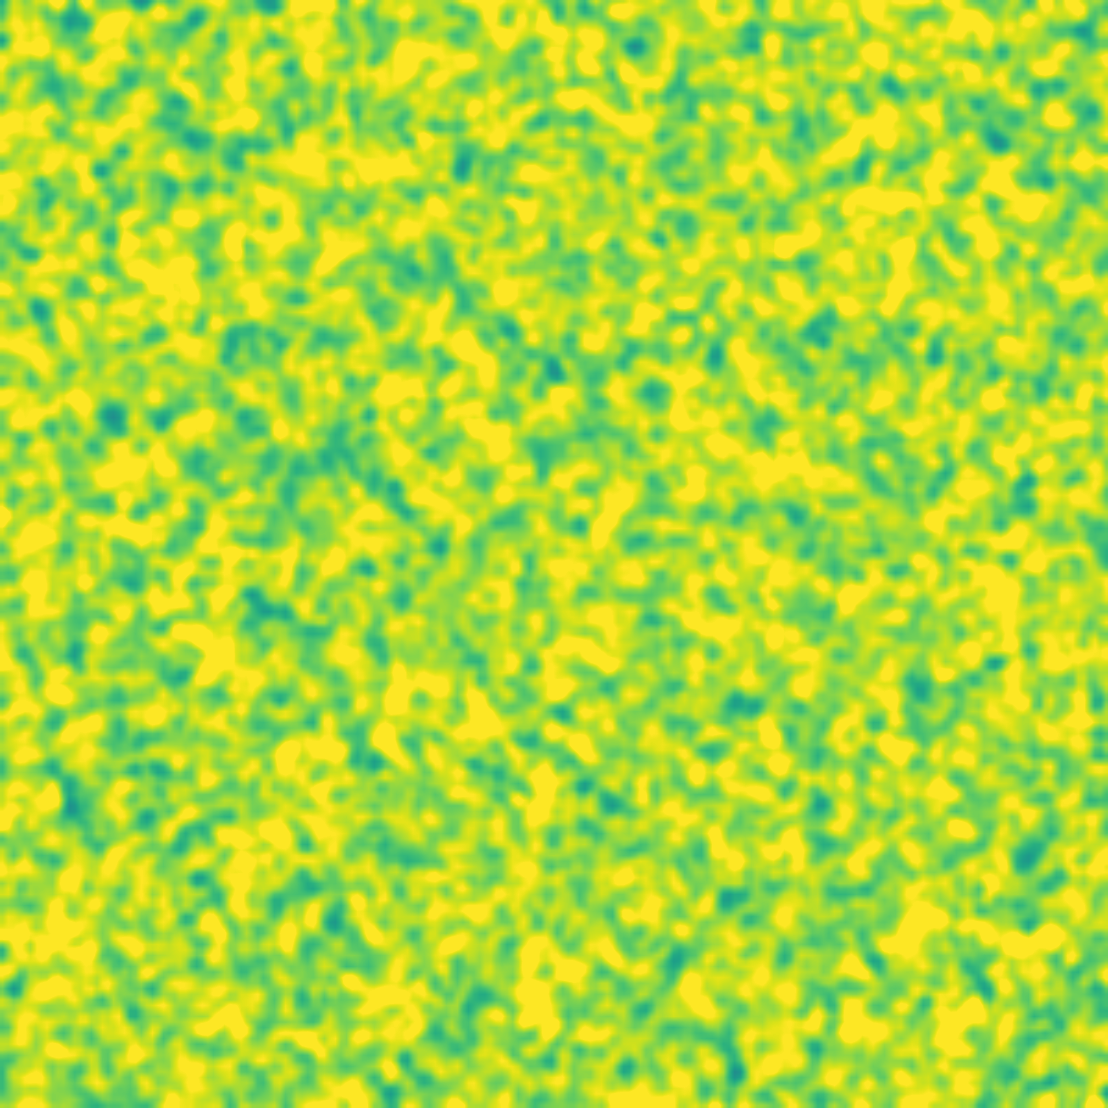
\includegraphics[width=0.32\linewidth]{papers/reaktdiff/images/simpleExample/easy_n1.png}
    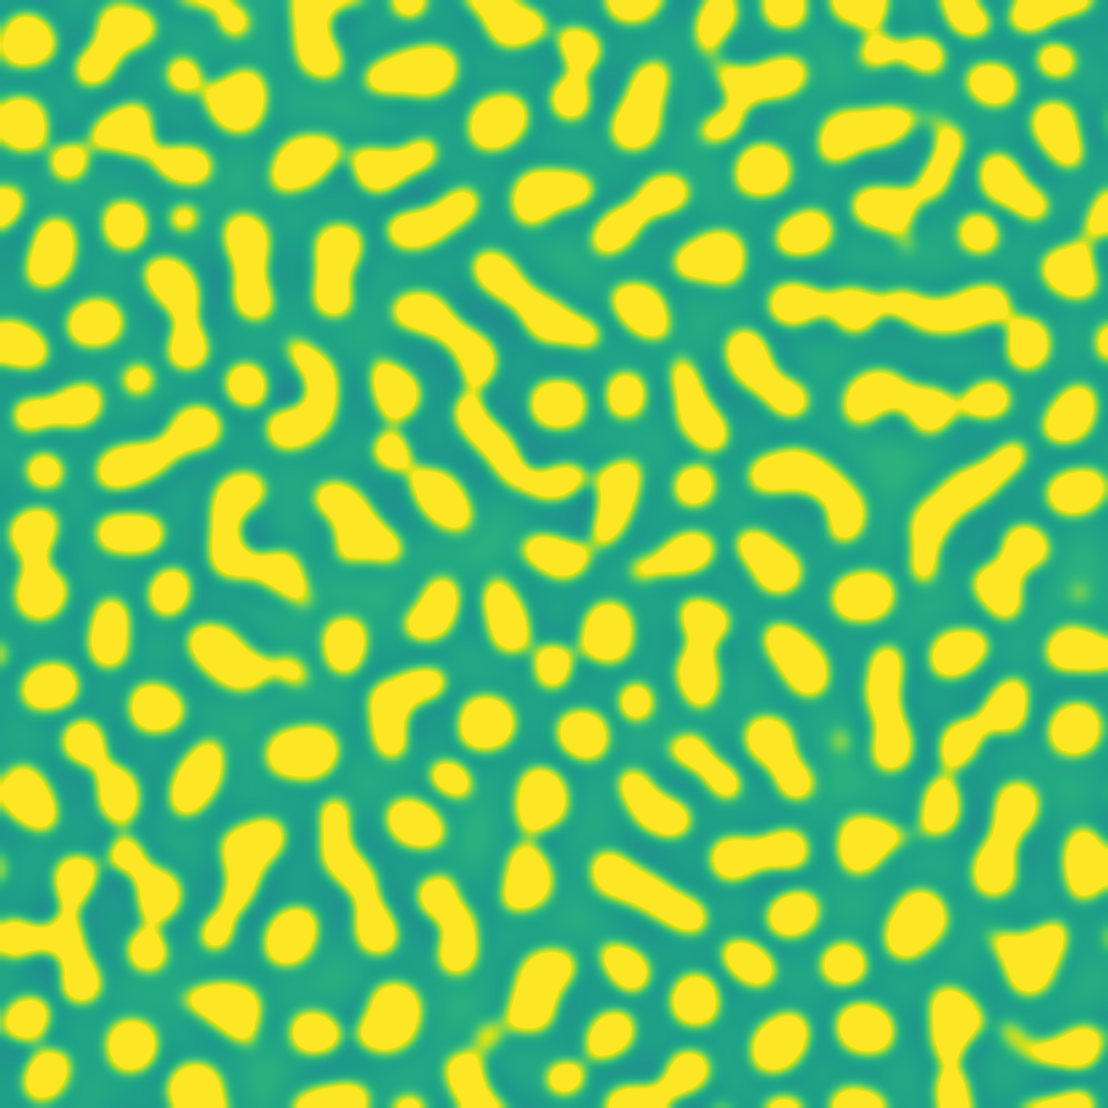
\includegraphics[width=0.32\linewidth]{papers/reaktdiff/images/simpleExample/easy_n300.png}
    
\includegraphics[width=0.32\linewidth]{papers/reaktdiff/images/simpleExample/easy_n999.png}
    \caption{Verlauf der Simulation (links nach rechts) der Reaktions-Diffusiongleichung mit \eqref{reaktdiff:equ:ownreakterm} als Reaktionsterm}
    \label{reaktdiff:fig:ownreakterm}
\end{figure}

\begin{figure}
    \centering
    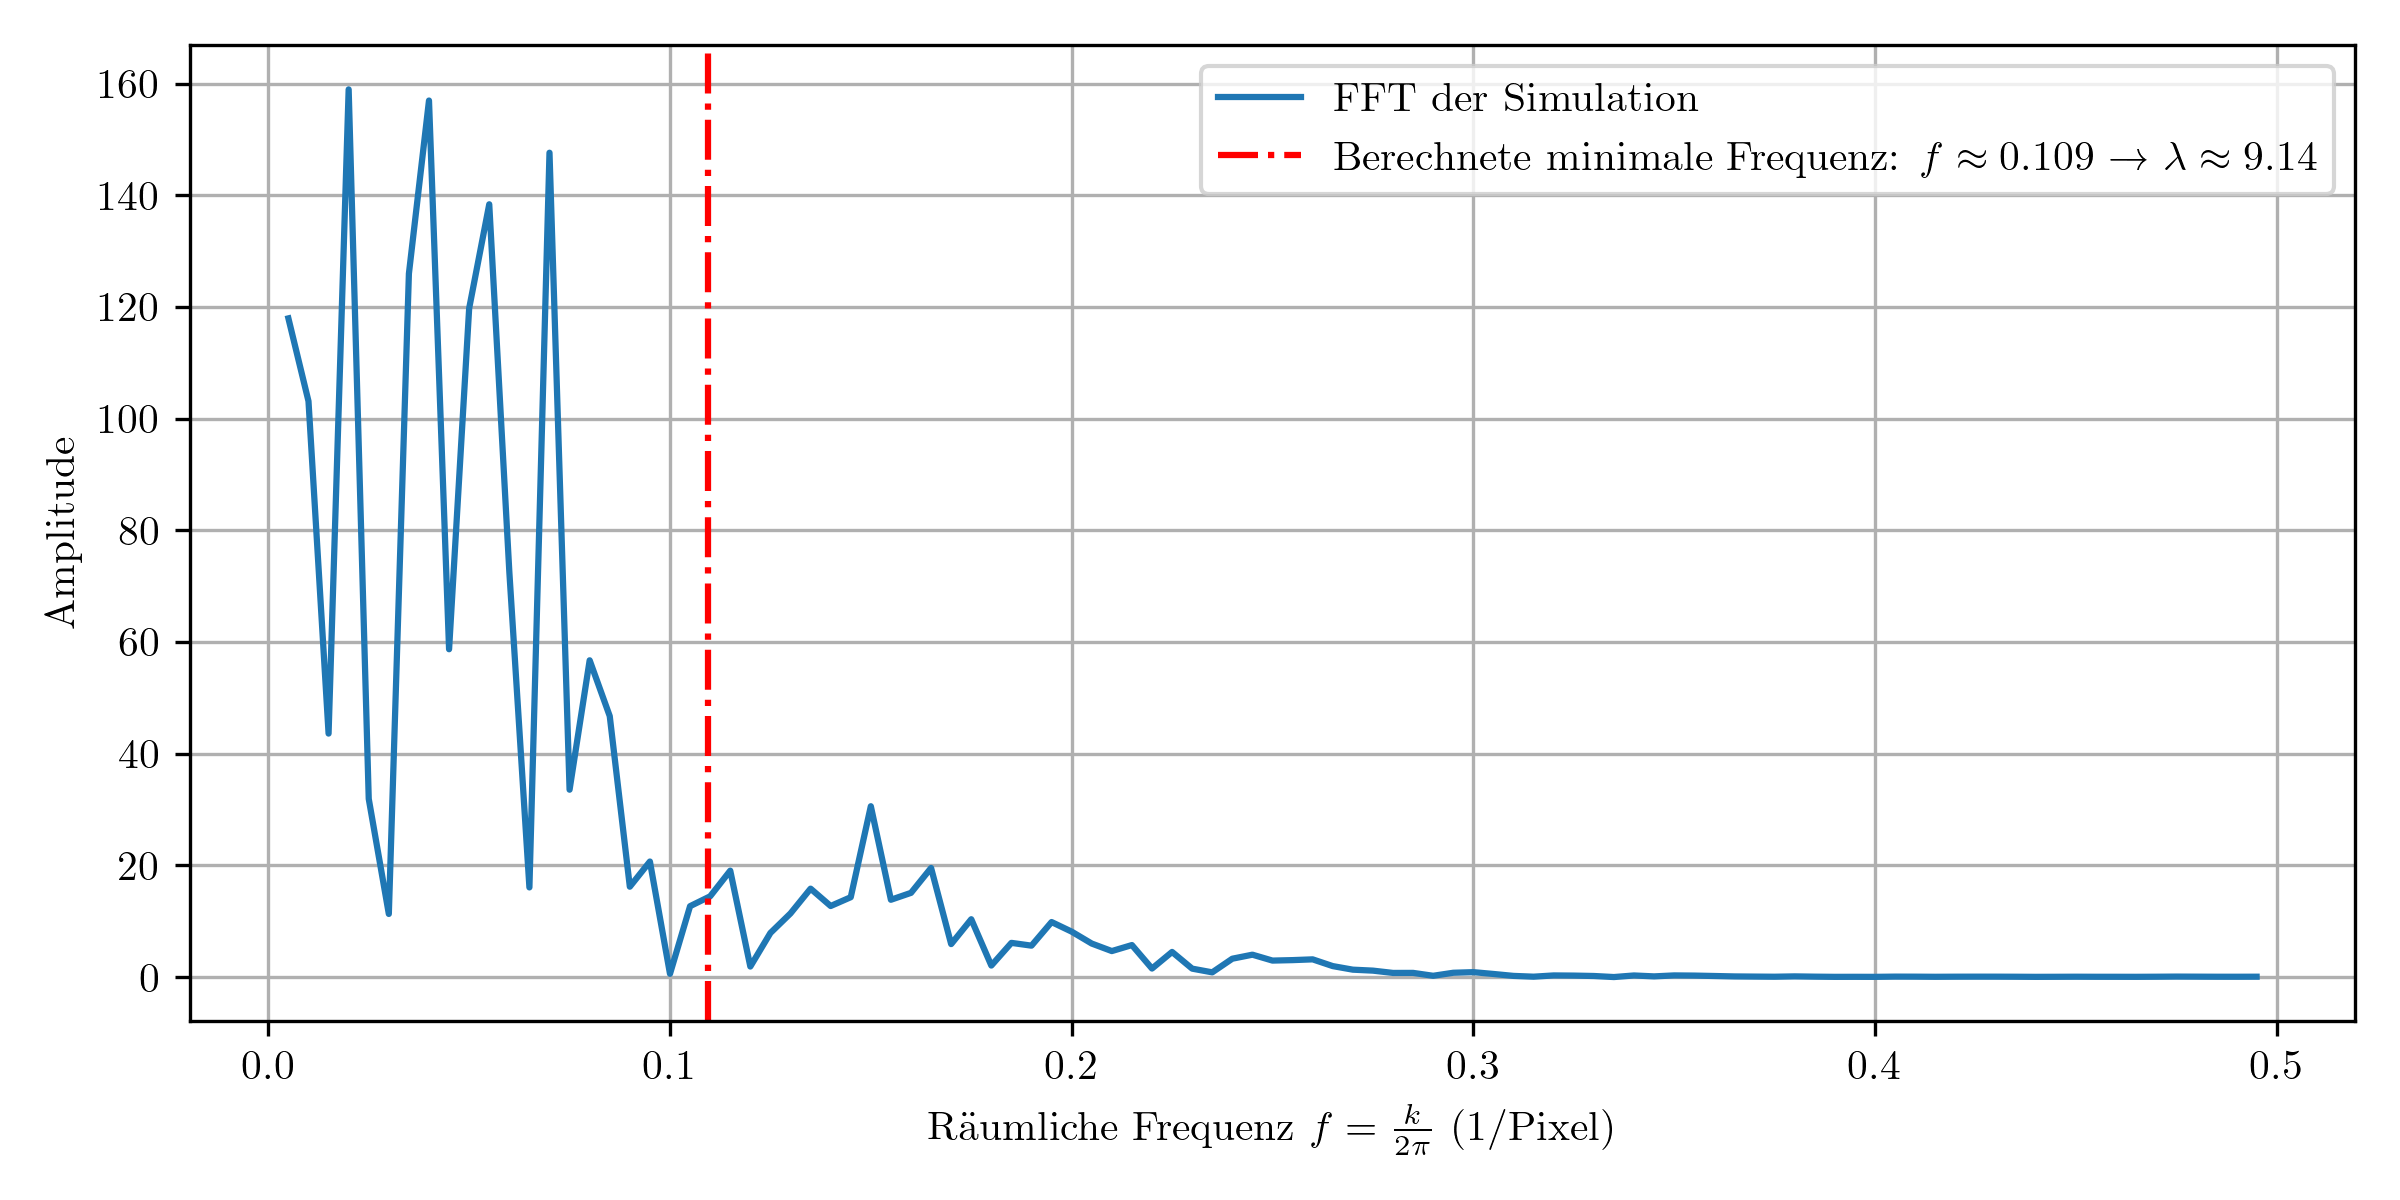
\includegraphics[width=\linewidth]{papers/reaktdiff/images/simpleExample/fft_turing_1d.png}
    \caption{FFT der Simulation eines Reaktionsdiffusionsmodell mit linearen Reaktionstermen \eqref{reaktdiff:equ:ownreakterm}. Die rote Linie zeigt die theortische minimale Frequnez von \(f = k_{\min} / 2 \pi \approx 0.109\). Man sieht, dass die dominanten Frequenzen links des berechneten Minimums ist.}
    \label{reaktdiff:fig:easyfft}
\end{figure}

%\begin{table}[h!]
%    \centering
%    \begin{tabular}{lcc}
%    \textbf{Größe} & \textbf{Theorie} & \textbf{Simulation (FFT)} \\
%    Dominante Frequenz $f$ (1/Pixel) & $\approx 0{,}075$ & $\approx 0{,060$ \\
%    Wellenlänge $\lambda = 1/f$ (Pixel) & $\approx 13{,}33$ & $\approx 16{,}67$ \\
%    Wellenzahl $k = 2\pi / \lambda$ & $\approx 0{,}472$ & $\approx 0{,}377$ \\
%    \end{tabular}
%    \caption{Vergleich zwischen theoretischer und numerisch bestimmter dominanter Wellenlänge. Die leichte Abweichung ist auf numerische Effekte der Simulation zurückzuführen.}
%    \label{tab:turing-vergleich}
%\end{table}



\subsection{Klassische Reaktionsterme}
In der Literatur werden viele weitere Reaktionsterme erwähnt.
Einige wenig werden hier im Anschluss beleuchtet.
Die folgenden Bilder zu den Modellen wurden mit der Finiten-Differenzen-Methode erstellt.

Als erstes wird das Gray-Scott Model berachtet.
Die Reaktionsterme
\begin{equation}
     f(u,v) = -uv^2 + F(1 - u), \quad g(u,v) = uv^2 - (F + k)v
     \label{reaktdiff:equ:gs}
\end{equation}
fördern wurmartige Muster.
Ein Beispiel kann in Abbildung \ref{reaktdiff:fig:gs} gesehen werden.


Ein weiteres Model ist das FitzHugh-Nagumo Model.
Es wird genutzt, um unter anderem die ausbreitung von Nervenimpulsen zu simulieren.
Die Reaktionsterme
\begin{equation}
    f(u,v) = \lambda_u u - u^3 - \kappa - \sigma v, \quad g(u,v) = \frac{1}{\tau}(u - v)
    \label{reaktdiff:equ:fhn}
\end{equation}
bilden Muster, welche man in der Natur bei Tieren sehen kann.
Ein Beispiel ist in Abbildung \ref{reaktdiff:fig:fhn} zu sehen.

\begin{figure}
    \centering
    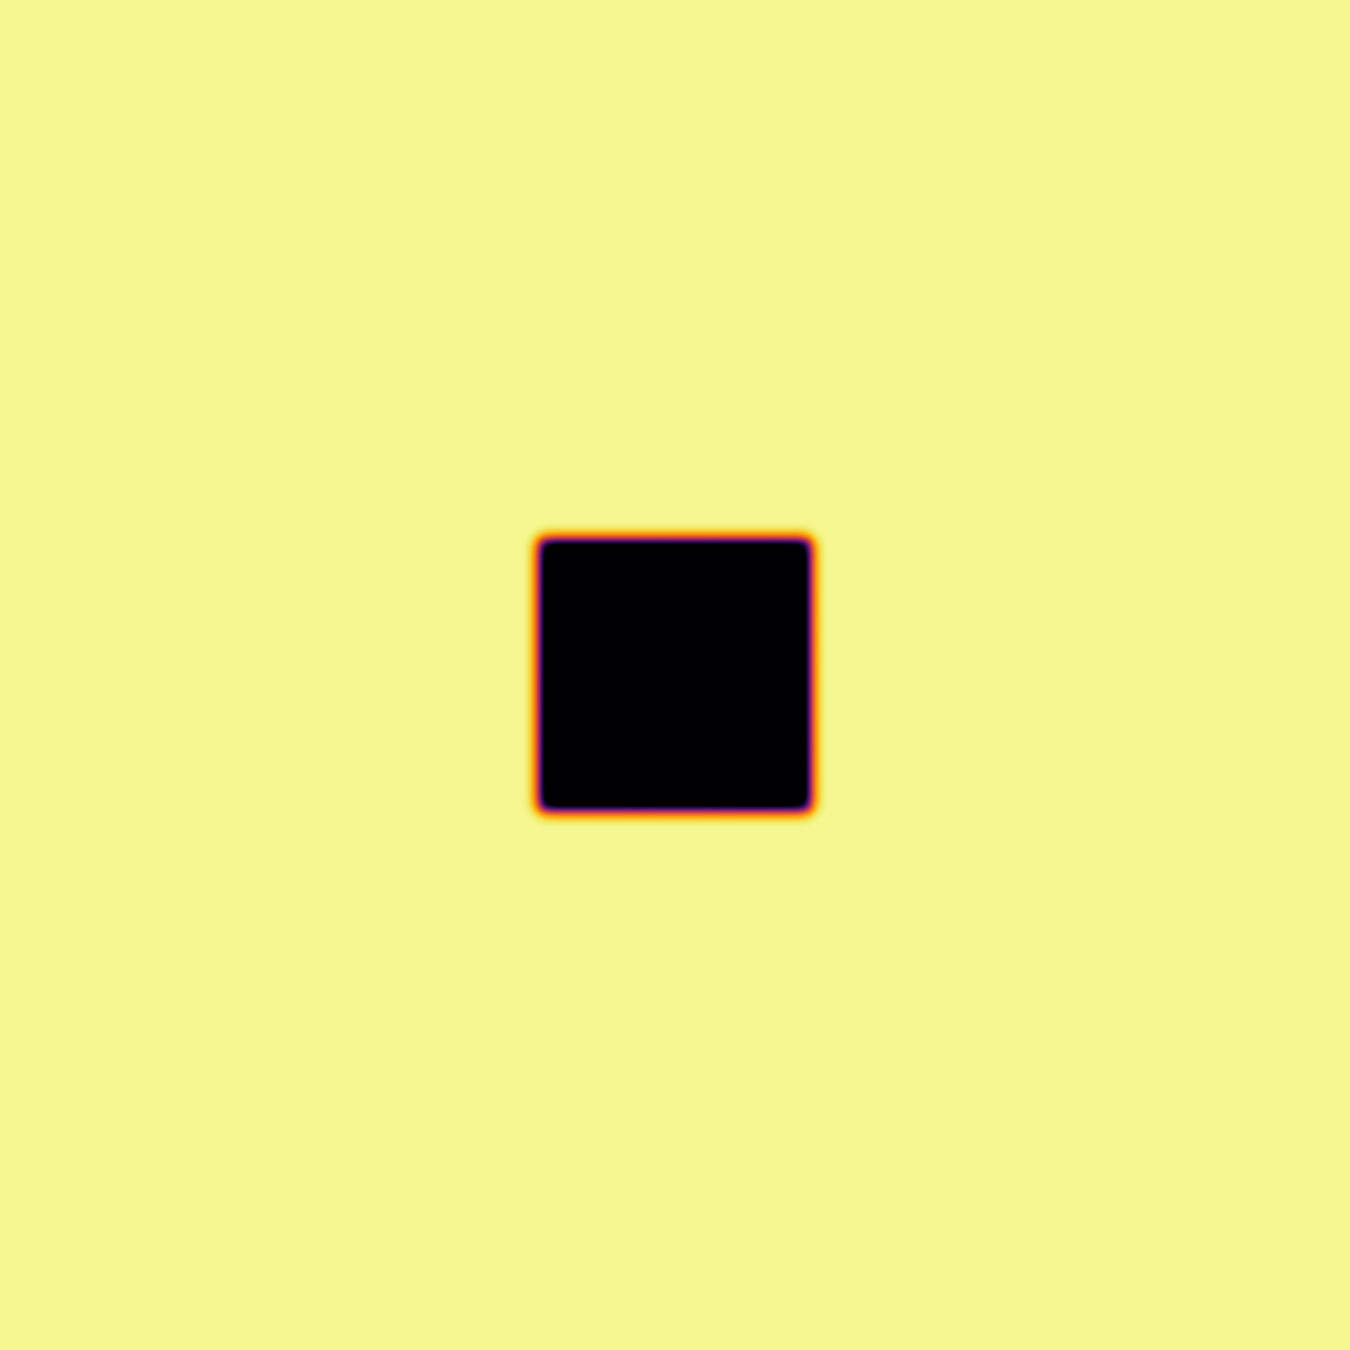
\includegraphics[width=0.32\linewidth]{papers/reaktdiff/images/GrayScott/gs_n1.png}
    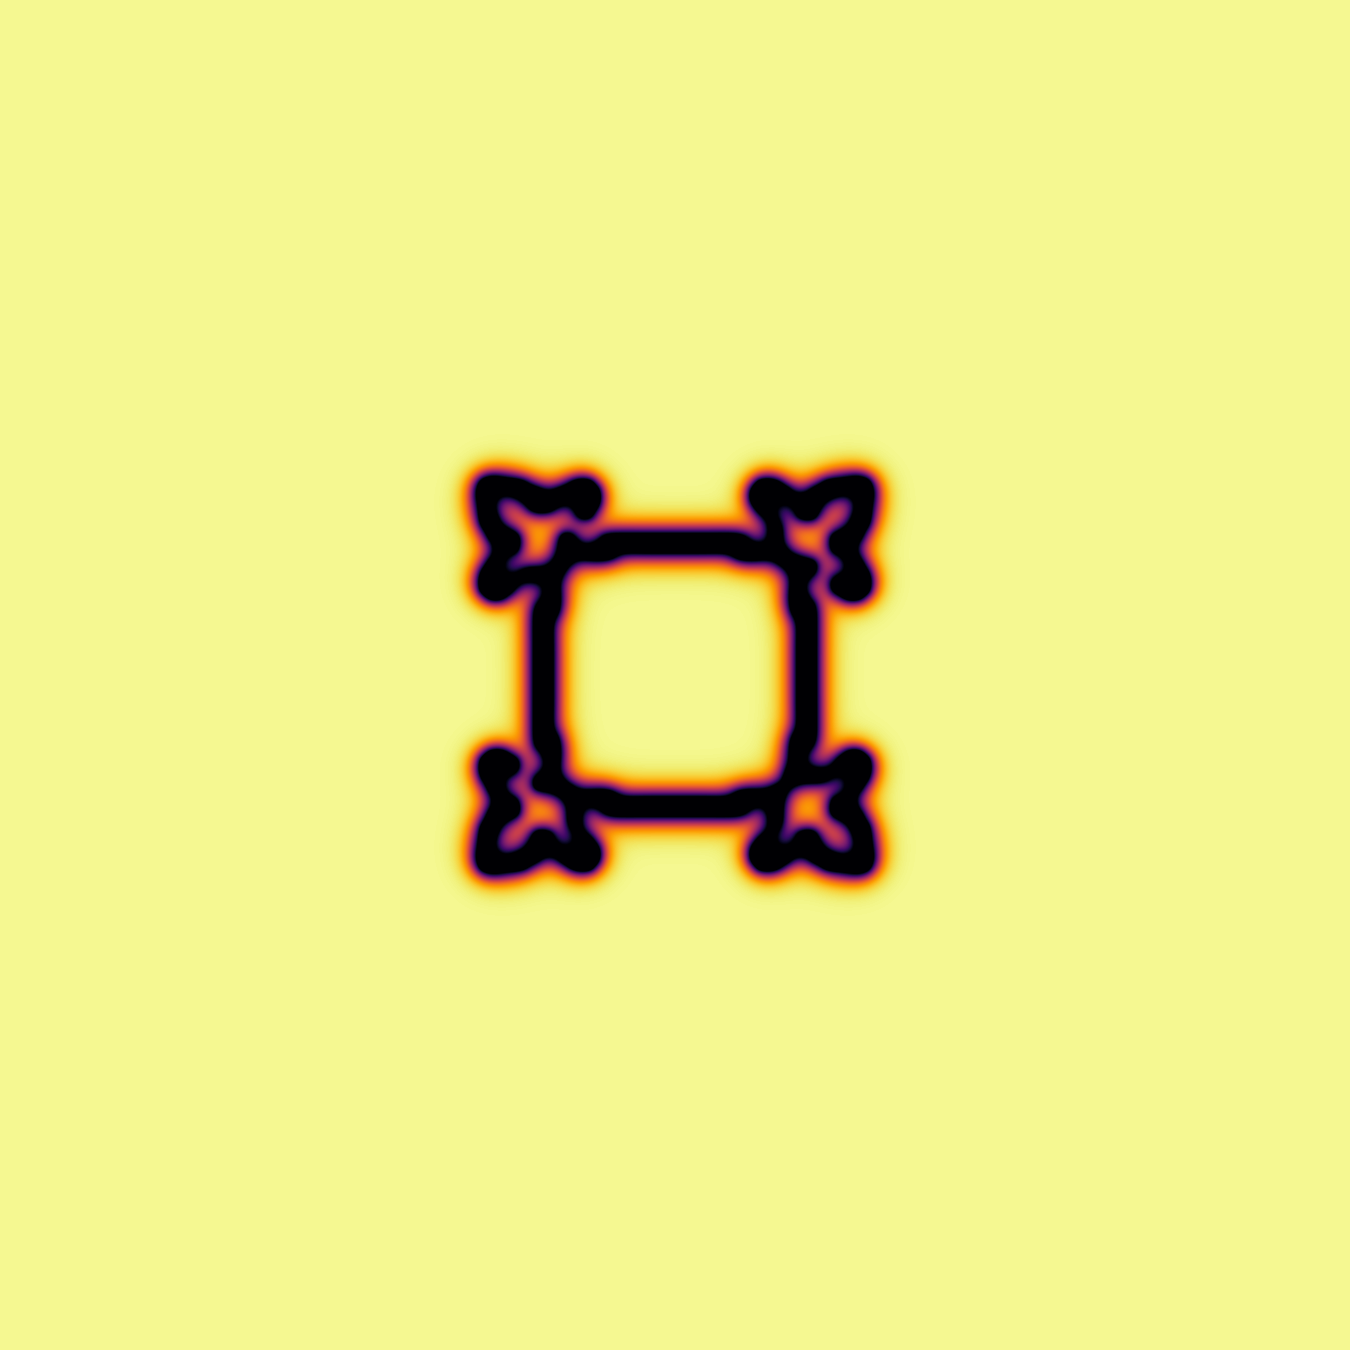
\includegraphics[width=0.32\linewidth]{papers/reaktdiff/images/GrayScott/gs_n300.png}
    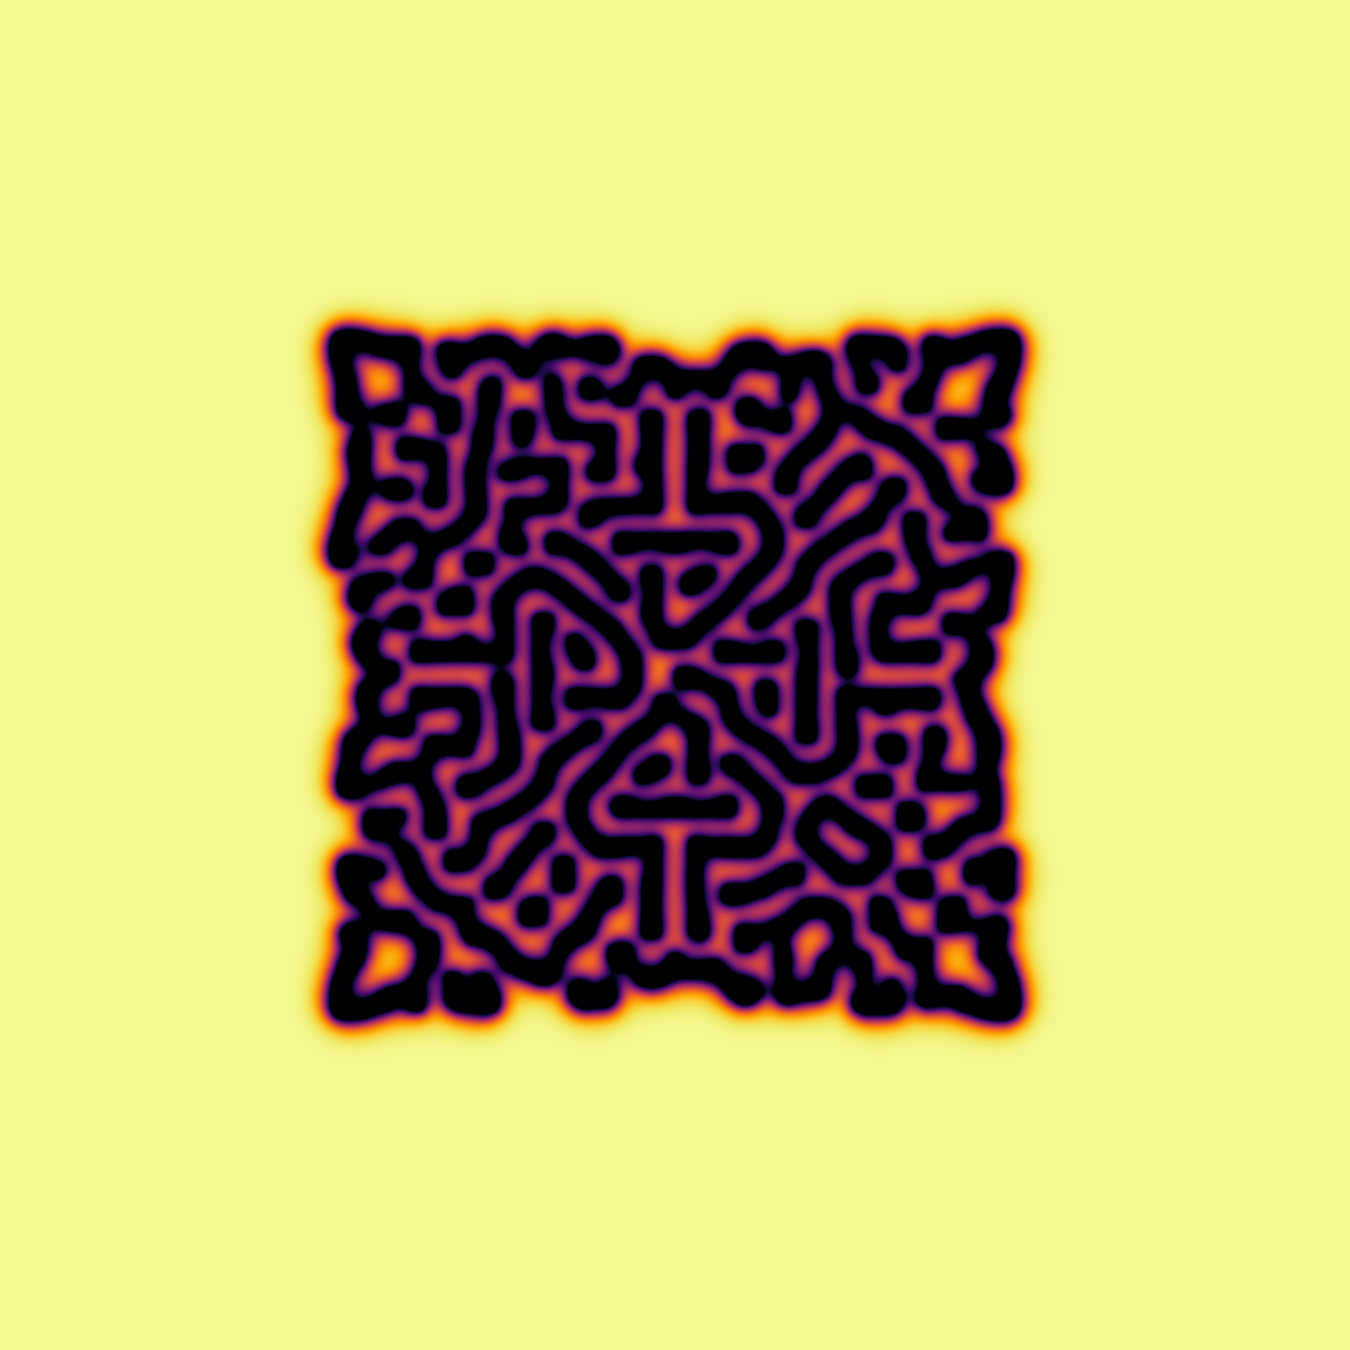
\includegraphics[width=0.32\linewidth]{papers/reaktdiff/images/GrayScott/gs_n999.png}
    \caption{Verlauf der Simulation (links nach rechts) der Reaktions-Diffusiongleichung mit Gray-Scott Modell (Gleichung \eqref{reaktdiff:equ:gs}) als Reaktionsterm.}
    \label{reaktdiff:fig:gs}
\end{figure}

\begin{figure}
    \centering
    
\includegraphics[width=0.32\linewidth]{papers/reaktdiff/images/FitzHughNagumo/fhn_n1.png}
    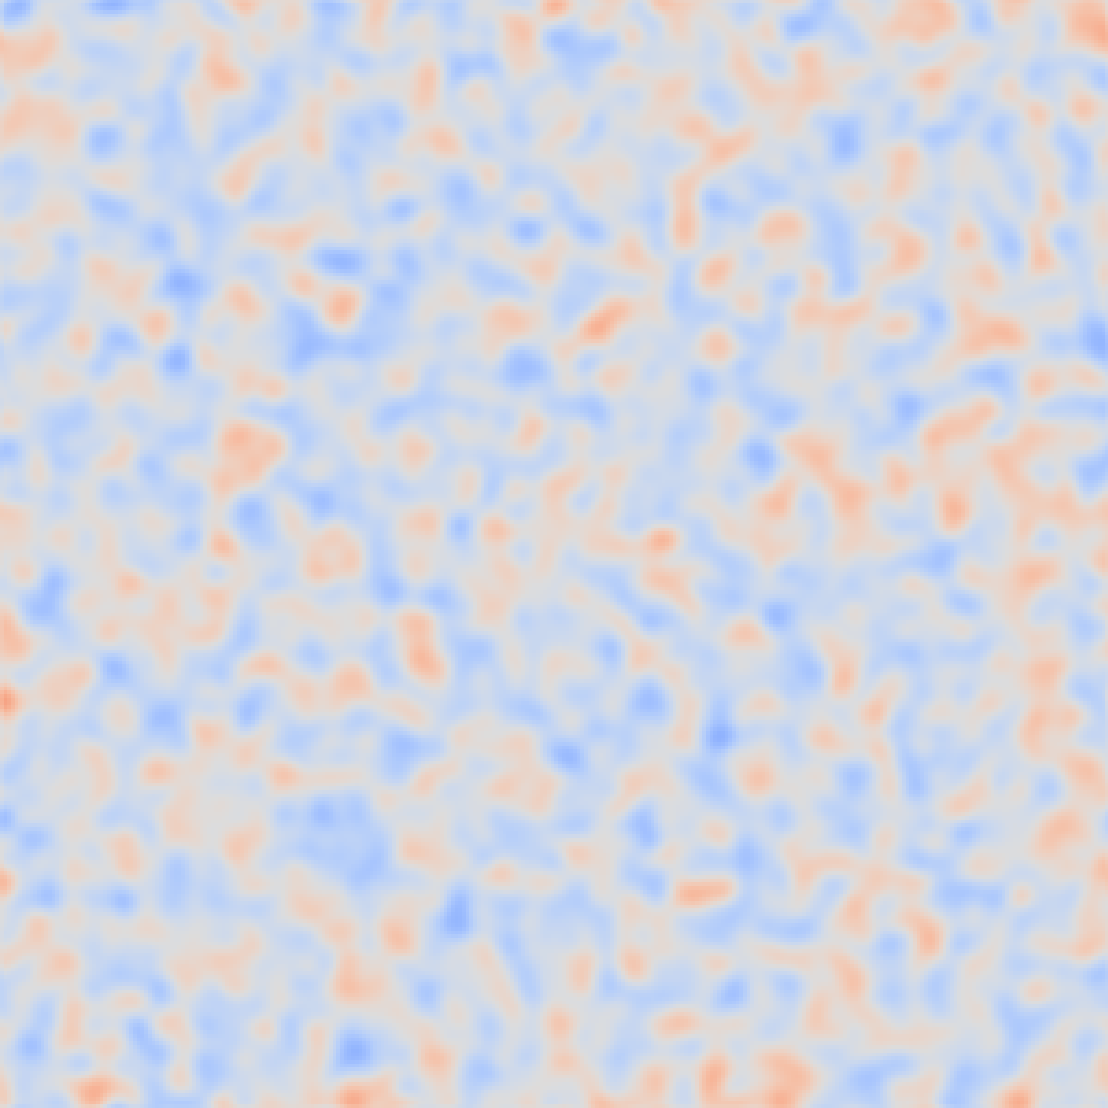
\includegraphics[width=0.32\linewidth]{papers/reaktdiff/images/FitzHughNagumo/fhn_n300.png}
    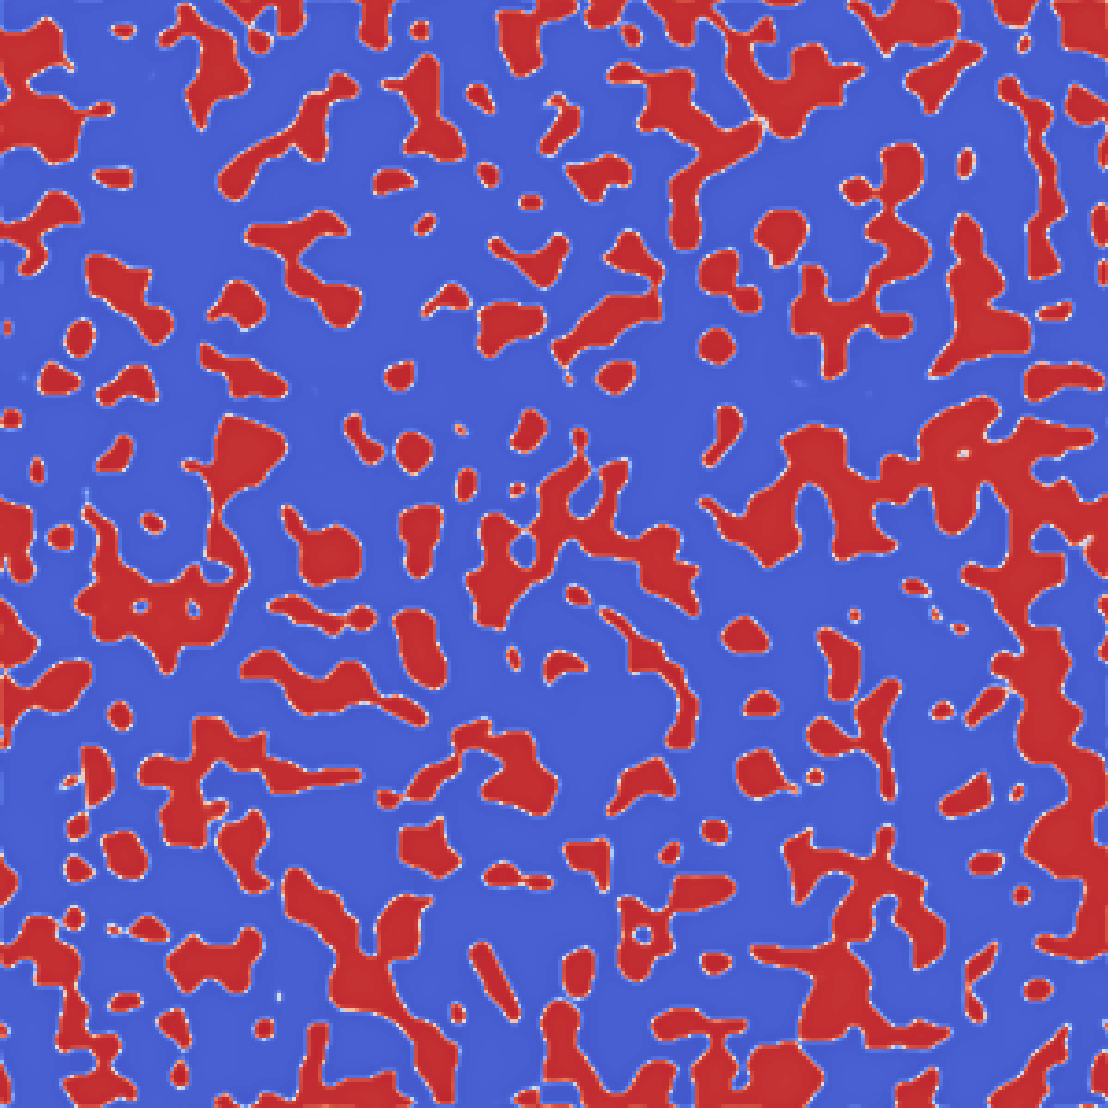
\includegraphics[width=0.32\linewidth]{papers/reaktdiff/images/FitzHughNagumo/fhn_n999.png}
    \caption{Verlauf der Simulation (links nach rechts) der Reaktions-Diffusiongleichung mit FitzHugh-Nagumo Modell (Gleichung \eqref{reaktdiff:equ:fhn}) als Reaktionsterm.}
    \label{reaktdiff:fig:fhn}
\end{figure}